\definecolor{mygreen}{rgb}{0,0.6,0}
\definecolor{mygray}{rgb}{0.5,0.5,0.5}
\definecolor{mymauve}{rgb}{0.58,0,0.82}

\lstset{ %
  backgroundcolor=\color{white},   % choose the background color; you must add \usepackage{color} or \usepackage{xcolor}
  % basicstyle=\footnotesize,        % the size of the fonts that are used for the code
  % breakatwhitespace=false,         % sets if automatic breaks should only happen at whitespace
  % breaklines=true,                 % sets automatic line breaking
  captionpos=b,                    % sets the caption-position to bottom
  % commentstyle=\color{mygreen},    % comment style
  % deletekeywords={...},            % if you want to delete keywords from the given language
  % %escapeinside={\%*}{*)},          % if you want to add LaTeX within your code
  % %extendedchars=true,              % lets you use non-ASCII characters; for 8-bits encodings only, does not work with UTF-8
  % %frame=single,	                % adds a frame around the code
  keepspaces=true,                 % keeps spaces in text, useful for keeping indentation of code (possibly needs columns=flexible)
  keywordstyle=\color{blue},       % keyword style
  % language=[ANSI]C,                % the language of the code
  % %otherkeywords={*,...},           % if you want to add more keywords to the set
  % numbers=left,                    % where to put the line-numbers; possible values are (none, left, right)
  numbersep=5pt,                   % how far the line-numbers are from the code
  numberstyle=\tiny\color{mygray}, % the style that is used for the line-numbers
  % rulecolor=\color{black},         % if not set, the frame-color may be changed on line-breaks within not-black text (e.g. comments (green here))
  % showspaces=false,                % show spaces everywhere adding particular underscores; it overrides 'showstringspaces'
  % showstringspaces=false,          % underline spaces within strings only
  % showtabs=false,                  % show tabs within strings adding particular underscores
  stepnumber=1,                    % the step between two line-numbers. If it's 1, each line will be numbered
  % stringstyle=\color{mymauve},     % string literal style
  % tabsize=2,	                   % sets default tabsize to 2 spaces
  title=\lstname,                  % show the filename of files included with \lstinputlisting; also try caption instead of title
  % morecomment=[s]{/*}{*/}
}

\chapter{Ensayos y Resultados}\label{Chapter4}

El capítulo muestra las pruebas de verificación realizadas en el trabajo,
herramientas utilizadas, resultados obtenidos y dificultades que se presentaron
durante el desarrollo.

% \section{Infraestructura para el Desarrollo}
% \section{Sintesis y recursos}

\section{Resultados obtenidos}

  En el marco del trabajo se ha logrado implementar con éxito un módulo SDI,
  el cual ha demostrado un funcionamiento conforme la gran mayoría de
  las expectativas planteadas inicialmente.
  % Este módulo se diseñó para facilitar
  % la transmisión de video en estándares SD-SDI, HD-SDI y 3G-SDI, cumpliendo con
  % los requerimientos de alta fiabilidad y eficiencia en el procesamiento de señales
  % de video digital de alta definición.

  En cuanto a los requerimientos específicos establecidos al inicio del trabajo,
  se han cumplido satisfactoriamente los siguientes puntos:

  \begin{enumerate}
      \item \textbf{Verificación:}
      \begin{enumerate}
          \item Se han realizado pruebas unitarias para cada módulo funcional,
          asegurando su correcto funcionamiento de manera aislada.
          \item Se ha llevado a cabo la simulación de bloques de protocolo
          completos y del sistema en su conjunto, haciendo una conexión en
          \textit{loopback} entre el transmisor y el receptor.
      \end{enumerate}
      \item \textbf{Funcionalidad:}
      \begin{enumerate}
          \item El módulo logra obtener las tasas de datos requeridas para los
          estándares SD-SDI\@.
          \item Se ha diseñado un sistema libre de problemas de \textit{timing}
          entre dominios de reloj y sin errores de \textit{setup} o \textit{hold}
          en las señales de entrada y salida.
          \item La implementación utiliza menos de 3000 \textit{Logic Array Blocks}
          en la FPGA, cumpliendo con los límites de recursos propuestos.
      \end{enumerate}
      \item \textbf{Metodología de trabajo:}
      \begin{enumerate}
          \item Se ha seguido un control de versiones riguroso utilizando Git,
          facilitando la gestión del código fuente y la colaboración entre los
          desarrolladores.
          \item El desarrollo se ha compilado y probado al menos en instancia final
          en Quartus y ModelSim, mientras que se desarrolló y verificó con
          herramientas \textit{open source} en la gran mayoría de los casos.
          \item La planificación y documentación del proyecto se ha gestionado a
          través de GitHub.
      \end{enumerate}
      \item \textbf{Documentación:}
      \begin{enumerate}
          \item Se ha elaborado una memoria técnica detallada, documentación de
          diseño y documentación de uso del módulo en GitHub, proporcionando un
          marco completo para su implementación y operación.
      \end{enumerate}
  \end{enumerate}

\section{Recursos utilizados}

  La tabla~\ref{tab:propio} lista el uso de recursos que utilizó el módulo SDI según el modo
  configurado en modo diferencial (con receptor y transmisor) no es un caso real
  de uso, pero sirve para comparar con la hoja de datos de Altera, que fue la
  referencia para este diseñó. El \textit{bitfile} fue generando con Altera
  Quartus II 15.0 por la misma razón.

  % \begin{center}
    \begin{table}[h]
      \centering
      \caption{Recursos utilizados por el módulo diseñado.}\label{tab:propio}
      \begin{tabular}{lcc}
        \toprule
        Modo & ALUTs combinacionales & Registros lógicos \\
        \hline
        SD-SDI & 1725 & 1164 \\
        \hline
        HD-SDI y 3G HD-SDI & 2237 & 1419 \\
        \hline
        Triple standard & 2753 & 2301 \\
        \bottomrule
        \hline
      \end{tabular}
    \end{table}
    % \end{center}

  Se identificó un problema en la compilación que causa que los módulos HD y 3G utilicen
  la misma cantidad de recursos, se sospecha que esto se debe a que cuando se instancia el
  módulo en formato HD se está instanciando el 3G con el \textit{transceiver}
  configurado a menor velocidad. Además, según la tabla~\ref{tab:propio} sale que se cumple con el
  requerimiento de ocupar menos de 3000 \textit{Logic Array Blocks} en la FPGA\@.

  Se hizo la tabla~\ref{tab:propio} para comparar con la que da la hoja de datos del
  dispositivo que se busca remplazar, tabla~\ref{tab:altera}.

  % \begin{center}
    \begin{table}[h]
      \centering
      \caption{Recursos utilizados por el módulo de Altera.}\label{tab:altera}
      \begin{tabular}{lcc}
        \toprule
        Modo & ALUTs combinacionales & Registros lógicos \\
        \hline
        SD-SDI & 1410 & 976 \\
        \hline
        HD-SDI & 1673 & 1063 \\
        \hline
        3G HD-SDI & 1673 & 1063 \\
        \hline
        Dual-Link HD-SDI & 2351 & 1696 \\
        \hline
        Dual standard receiver & 1539 & 1042 \\
        \hline
        Dual standard transmitter & 352 & 260 \\
        \hline
        Triple standard & 2421 & 1805 \\
        \bottomrule
        \hline
      \end{tabular}
    \end{table}
  % \end{center}

  Se puede observar comparando ambas tablas, que el módulo original tiene varios
  modos más que el desarrollado en este trabajo, pero estos modos no habían sido
  contemplados en el trabajo ya que en la empresa VideoSwitch no se usan. Además,
  se puede apreciar que el módulo original ocupa menos recursos en todos los
  modos, pero en todos los casos está en el mismo orden.

% \section{Funcionamiento operativo}

\section{Pruebas unitarias}

  En la presente sección del documento se muestran únicamente algunos ejemplos de
  todas las pruebas unitarias realizadas. Estas muestras representan una fracción
  de la totalidad de pruebas unitarias llevadas a hechas durante el desarrollo del
  trabajo. Se optó por incluir estos casos de prueba como ejemplos representativos
  para ilustrar el proceso de verificación, ya que contando con más de 20 módulos
  cada uno con multiples configuraciones no se consideró útil enriquecedor agregar
  todos los casos.

  Es importante destacar que el conjunto completo de pruebas unitarias, así como
  otros aspectos relacionados con el desarrollo y la implementación, están
  disponibles de forma completa en los \textit{pipeline} de CI de GitHub del
  proyecto. Este repositorio, al ser público, proporciona acceso a todos los
  detalles relevantes del proceso de desarrollo, incluidas las pruebas unitarias
  completas, las funcionales, las de integración a nivel sistema, los \textit{linter}
  y otros aspectos relevantes del flujo de trabajo de desarrollo~\citep{github}.

  Por lo tanto, para una visión exhaustiva y detallada de las pruebas unitarias
  y otros elementos del proyecto, se recomienda consultar el \textit{pipeline} de
  GitHub correspondiente, donde se encuentran disponibles de manera más adecuada
  para un análisis completo en el contexto de una tesis.

% todo: AGREGAR LINK!!!!!

\subsection{Replicador de bits}

  Se corrieron las pruebas unitarias del replicador de bits:

  % {\tiny\begin{verbatim}
  {\tiny\begin{lstlisting}[caption= "Resultados \textit{test} replicador de bits.]
    Seeding Python random module with 1709476252
    Found test test_sdi_bit_rep.test_sdi_bit_rep
    running test_sdi_bit_rep (1/1)
    test_sdi_bit_rep passed
    *******************************************************************************************
    ** TEST                               STATUS  SIM TIME (ns)  REAL TIME (s)  RATIO (ns/s) **
    *******************************************************************************************
    ** test_sdi_bit_rep.test_sdi_bit_rep   PASS         300.00           0.00     192723.42  **
    *******************************************************************************************
    ** TESTS=1 PASS=1 FAIL=0 SKIP=0                     300.00           0.03       9765.47  **
    *******************************************************************************************
  \end{lstlisting}}
  % \end{verbatim}}

  La simulación del módulo bit\_rep se realizó con éxito, confirmando el correcto
  funcionamiento del diseño. Durante la simulación, se observó que el módulo
  replicaba los bits de los datos de entrada 11 veces, ver figura~\ref{fig:bit-rep},
  generando una salida de 20 bits en cada ciclo de reloj.

  \begin{figure}[htbp]
    \centering
    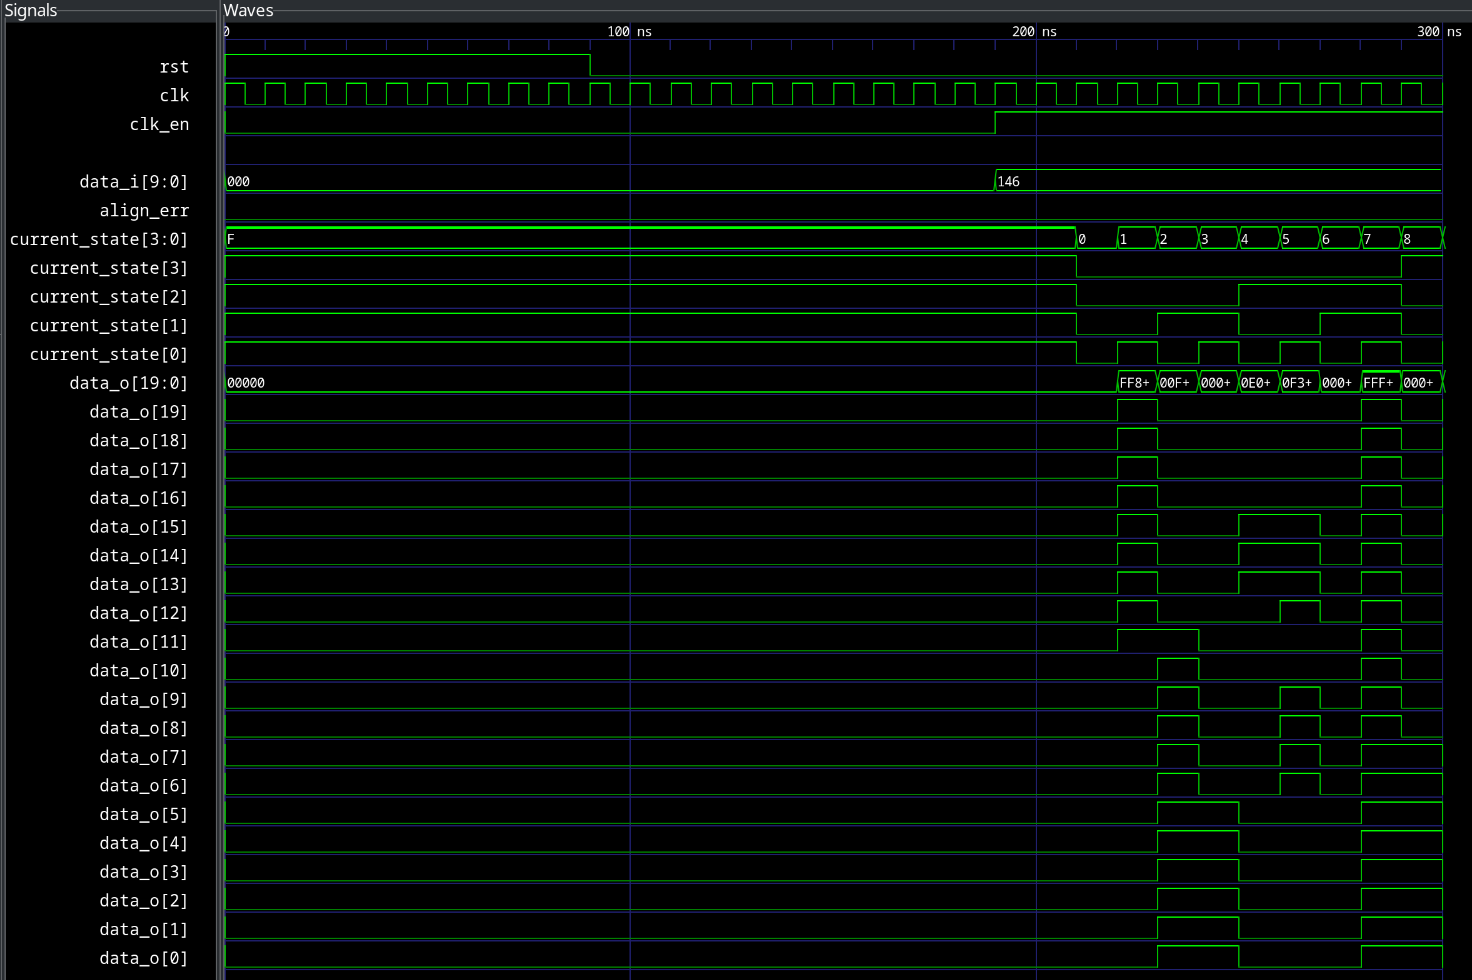
\includegraphics[width=1\textwidth]{./Figures/bit_rep.png}
    \caption{Simulación del módulo bit\_rep.}\label{fig:bit-rep}
  \end{figure}
  
  Se verificó que la máquina de estados se alineaba automáticamente, garantizando
  un comportamiento adecuado independientemente de la cadencia inicial del reloj
  de habilitación. Además, no se detectaron desalineaciones en la cadencia 5/6/5/6
  durante la simulación. Estos resultados validan la funcionalidad esperada del
  módulo.

\subsection{Verificación de redundancia cíclica}

  {\tiny\begin{lstlisting}[caption= "Resultados \textit{test} inserción de redundancia cíclica.]
    Seeding Python random module with 1709474689
    Found test test_crc_insert.crc_insert_test
    running crc_insert_test (1/1)
    crc_insert_test passed
    *****************************************************************************************
    ** TEST                             STATUS  SIM TIME (ns)  REAL TIME (s)  RATIO (ns/s) **
    *****************************************************************************************
    ** test_crc_insert.crc_insert_test   PASS         430.36           0.00     244532.75  **
    *****************************************************************************************
    ** TESTS=1 PASS=1 FAIL=0 SKIP=0                   430.36           0.03      14103.80  **
    *****************************************************************************************
  \end{lstlisting}}

  Se corrieron las respectivas pruebas unitarias, tanto para el módulo capaz de
  calcular el CRC, como para los \textit{wrappers} que adaptan las señales del
  flujo transmisión y recepción de datos:

  {\tiny\begin{lstlisting}[caption= "Resultados \textit{test} recepción de redundancia cíclica.]
    Seeding Python random module with 1709474535
    Found test test_crc_rx.crc_rx_test
    running crc_rx_test (1/1)
    test_crc_rx passed
    **************************************************************************************
    ** TEST                          STATUS  SIM TIME (ns)  REAL TIME (s)  RATIO (ns/s) **
    **************************************************************************************
    ** test_crc_rx.crc_rx_test        PASS         489.01           0.00     218972.36  **
    **************************************************************************************
    ** TESTS=1 PASS=1 FAIL=0 SKIP=0                489.01           0.03      17432.87  **
    **************************************************************************************
  \end{lstlisting}}

  {\tiny\begin{lstlisting}[caption= "Resultados \textit{test} cálculo de redundancia cíclica.]
    Seeding Python random module with 1709473164
    Found test test_crc18.crc18_test
    running crc18_test (1/1)
    crc18_test passed
    **************************************************************************************
    ** TEST                          STATUS  SIM TIME (ns)  REAL TIME (s)  RATIO (ns/s) **
    **************************************************************************************
    ** test_crc18.crc18_test          PASS         390.63           0.00     250945.16  **
    **************************************************************************************
    ** TESTS=1 PASS=1 FAIL=0 SKIP=0                390.63           0.03      11570.77  **
    **************************************************************************************
  \end{lstlisting}}

  La simulación del módulo de verificación de redundancia cíclica se llevó a cabo
  con éxito, confirmando su correcto funcionamiento en la verificación del CRC,
  ver figuras~\ref{fig:crc18} y~\ref{fig:crc18-z}\@.

  \begin{figure}[htbp]
    \centering
    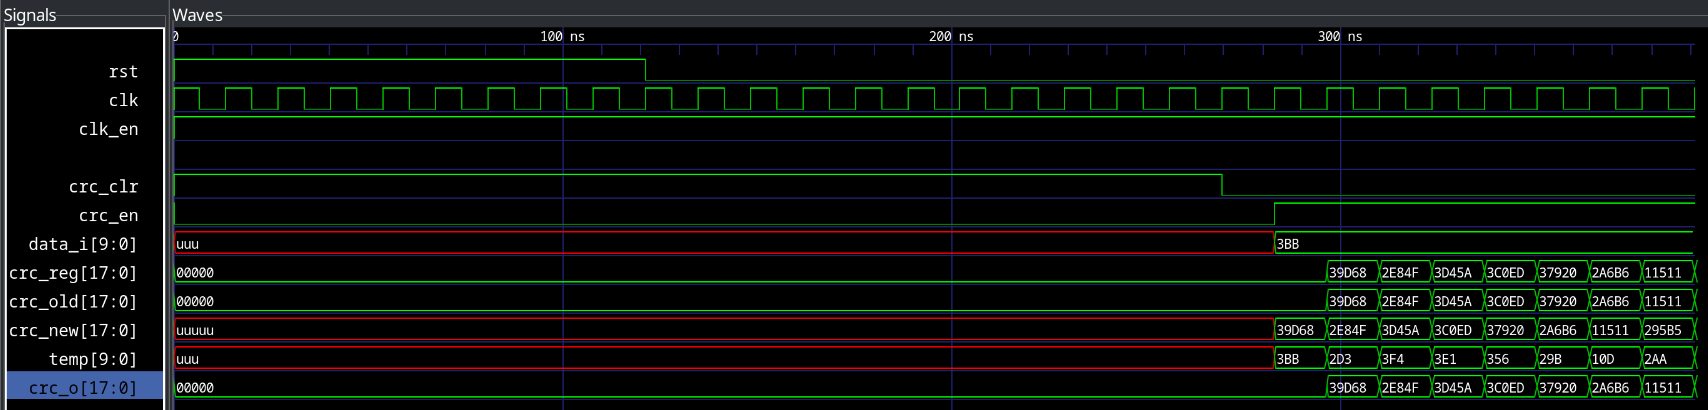
\includegraphics[width=1\textwidth]{./Figures/crc18.png}
    \caption{Simulación del módulo crc18.}\label{fig:crc18}
  \end{figure}

  Durante la simulación, se observó que el módulo calculaba correctamente el
  valor CRC para cada línea de video, tanto para los canales Y como para C.
  
  Además, se verificó que el valor CRC calculado se comparaba con el valor CRC
  recibido, activando la salida de error CRC correspondiente en caso de detectarse
  un error. Esta salida permaneció activada durante el tiempo de una línea de
  video, como se esperaba, hasta que se realizó la próxima verificación de CRC\@.

  \begin{figure}[htbp]
    \centering
    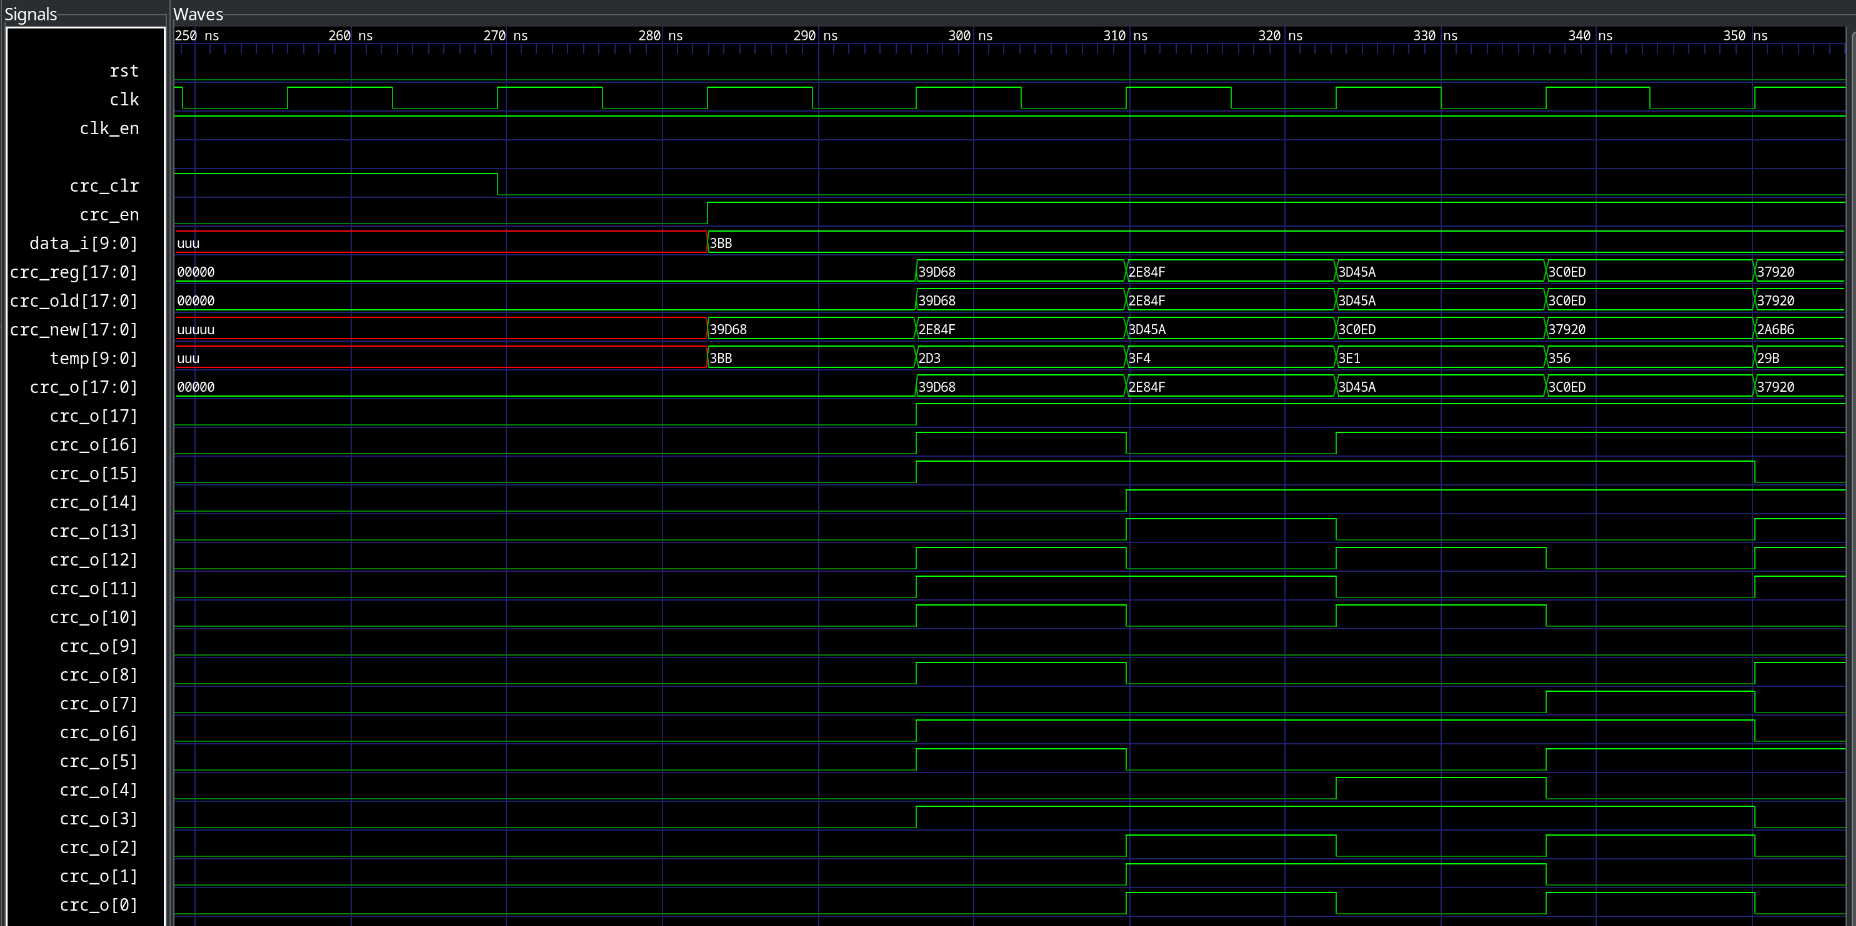
\includegraphics[width=1\textwidth]{./Figures/crc18_zoom.png}
    \caption{Simulación del módulo crc18 enfocada en los datos.}\label{fig:crc18-z}
  \end{figure}

  Adicionalmente, se pudo observar que el módulo capturaba correctamente los
  valores del número de línea para ambos canales y los emitía adecuadamente.
  Estos valores del número de línea fueron válidos durante todo el tiempo de la
  línea, como se especificaba en la descripción del módulo.

\subsection{Codificador}

  Se corrieron las pruebas unitarias del codificador y sus sus submódulos:

  {\tiny\begin{lstlisting}[caption= "Resultados \textit{test} de conversor NRZ a NRZI.]
    Seeding Python random module with 1709472961
    Found test test_nrz_2_nrzi.nrzi_basic_test
    running nrzi_basic_test (1/1)
    [1, 0, 0, 1, 1, 0, 0, 1, 1]
    [1, 0, 0, 1, 1, 0, 0, 1, 1]
    nrzi_basic_test passed
    *****************************************************************************************
    ** TEST                             STATUS  SIM TIME (ns)  REAL TIME (s)  RATIO (ns/s) **
    *****************************************************************************************
    ** test_nrz_2_nrzi.nrzi_basic_test   PASS         296.34           0.00     249286.01  **
    ** test_nrz_2_nrzi.nrzi_random_test  PASS         279.12           0.00     340029.54  **
    *****************************************************************************************
    ** TESTS=2 PASS=2 FAIL=0 SKIP=0                   575.46           0.02      16257.78  **
    *****************************************************************************************
  \end{lstlisting}}

  Durante la simulación, se observó que el módulo funcionaba correctamente.
  Convirtiendo los datos de entrada de la codificación NRZ a NRZI de manera
  adecuada. La señal de habilitación permitio activar o desactivar la
  conversión de manera correcta. Durante la simulación, se verificó que esta
  señal funcionara como se esperaba, controlando efectivamente la operación
  del convertidor.

  \begin{figure}[h]
    \centering
    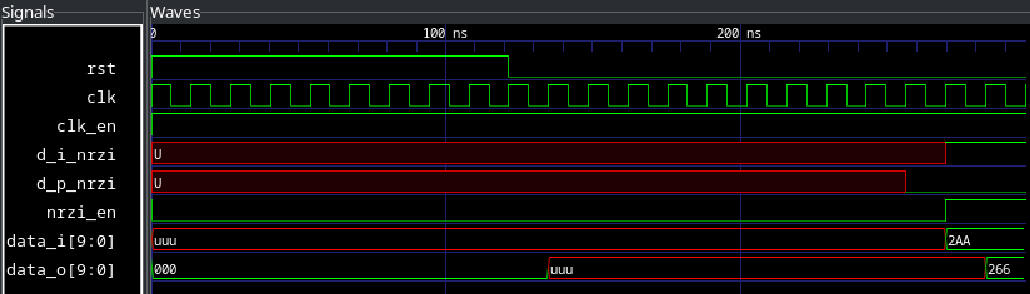
\includegraphics[width=1\textwidth]{./Figures/nrz2nrzi.png}
    \caption{Simulación del módulo nrz\_2\_nrzi.}\label{fig:nrzi}
  \end{figure}

  Se observó que el módulo es estable y no muestra comportamientos inesperados
  durante la simulación. No se observaron oscilaciones, estados intermedios
  inestables o glitches en las señales de salida. Los datos de salida del
  convertidor NRZ a NRZI se corresponden con los establecidos en el modelo de
  referencia.

  {\tiny\begin{lstlisting}[caption= "Resultados \textit{test} de \textit{scrambler}.]
    Seeding Python random module with 1836729247
    Found test test_scram_smpte.test_scram_smpte
    running test_scram_smpte (1/1)
    test_scram_smpte passed
    *****************************************************************************************
    ** TEST                             STATUS  SIM TIME (ns)  REAL TIME (s)  RATIO (ns/s) **
    *****************************************************************************************
    ** test_scram_smpte.test_scram_smpte PASS         412.87           0.00      318947.62 **
    *****************************************************************************************
    ** TESTS=1 PASS=1 FAIL=0 SKIP=0                   412.87           0.03       14427.10 **
    *****************************************************************************************
  \end{lstlisting}}

  Durante la simulación, se observó que el módulo funcionaba correctamente.
  Genera secuencias de bits scrambled según el estándar SMPTE\@.

  {\tiny\begin{lstlisting}[caption= "Resultados \textit{test} de \textit{encoder}.]
    Seeding Python random module with 287641029
    Found test test_sdi_enc.test_sdi_enc
    running test_sdi_enc (1/1)
    test_sdi_enc passed
    *****************************************************************************************
    ** TEST                             STATUS  SIM TIME (ns)  REAL TIME (s)  RATIO (ns/s) **
    *****************************************************************************************
    ** test_sdi_enc.test_sdi_enc         PASS         589.23           0.00      241846.07 **
    *****************************************************************************************
    ** TESTS=1 PASS=1 FAIL=0 SKIP=0                   589.23           0.04       14730.75 **
    *****************************************************************************************
  \end{lstlisting}}

  La simulación del decoder y encoder no fue trivial, debido a que el modelo
  no fue fácil de reproducir, de todas formas una vez que se encontró una
  biblioteca de Python, se observó que ambos módulos operaban correctamente.
  Procesa los datos de entrada según los estándares SDI y generaba datos
  de salida de manera adecuada.

  {\tiny\begin{lstlisting}[caption= "Resultados \textit{test} de \textit{decoder}.]
    Seeding Python random module with 1654987444
    Found test test_sdi_deco.test_sdi_deco
    running test_sdi_deco (1/1)
    test_sdi_deco passed
    *****************************************************************************************
    ** TEST                             STATUS  SIM TIME (ns)  REAL TIME (s)  RATIO (ns/s) **
    *****************************************************************************************
    ** test_sdi_deco.test_sdi_deco       PASS         212.58           0.00      196837.42 **
    *****************************************************************************************
    ** TESTS=1 PASS=1 FAIL=0 SKIP=0                   212.58           0.02        8576.24 **
    *****************************************************************************************
  \end{lstlisting}}

\subsection{Estándar SMPTE 292M \textit{framer}}

  Se observó que el módulo cumple con la norma durante la simulación.
  No se observaron oscilaciones, estados intermedios inestables o glitches en las
  señales de salida.

  {\tiny\begin{lstlisting}[caption= "Resultados \textit{test} de \textit{framer}.]
    Seeding Python random module with 2598374610
    Found test test_framer.test_framer
    running test_framer (1/1)
    test_framer passed
    *******************************************************************************************
    ** TEST                               STATUS  SIM TIME (ns)  REAL TIME (s)  RATIO (ns/s) **
    *******************************************************************************************
    ** test_framer.test_framer             PASS         325.00           0.01     187654.33  **
    *******************************************************************************************
    ** TESTS=1 PASS=1 FAIL=0 SKIP=0                     325.00           0.04       9587.13  **
    *******************************************************************************************
  \end{lstlisting}}

  En la siguientes tablas se puede apreciar uno de los casos simulados exitosamente.
  En la tabla~\ref{tab:in}, los datos \textit{unscrambled} de entrada y en la tabla~\ref{tab:out}, los
  datos de salida.

  % \begin{center}
    \begin{table}[h]
      \centering
      \caption{Datos de entrada.}
      \begin{tabular}{lccccc}
        \toprule
        Bits 18\-19 & 14\-17 & 10\-13 & 8\-9 & 4\-7 & 0\-3 \\ \hline
        11 & 1111 & 1111 & 11 & 11xx & xxxx \\ \hline
        00 & 0000 & 0000 & 00 & 0011 & 1111 \\ \hline
        00 & 0000 & 0000 & 00 & 0000 & 0000 \\ \hline
        aa & aaaa & aaaa & aa & aa00 & 0000 \\ \hline
        bb & bbbb & bbbb & bb & bbbb & bbbb \\ \hline
        cc & cccc & cccc & cc & cccc & cccc \\ \hline
        \bottomrule
        \hline
      \end{tabular}
      \label{tab:in}
    \end{table}
  % \end{center}

  % \begin{center}
    \begin{table}[h]
      \centering
      \caption{Datos de salida.}
      \begin{tabular}{lccccc}
        \toprule
        Bits 18\-19 & 14\-17 & 10\-13 & 8\-9 & 4\-7 & 0\-3 \\ \hline
        xx & xxxx & xxxx & xx & xxxx & xxxx \\ \hline
        11 & 1111 & 1111 & 11 & 1111 & 1111 \\ \hline
        00 & 0000 & 0000 & 00 & 0000 & 0000 \\ \hline
        00 & 0000 & 0000 & 00 & 0000 & 0000 \\ \hline
        bb & bbbb & aaaa & aa & aaaa & aaaa \\ \hline
        cc & cccc & bbbb & bb & bbbb & bbbb \\
        \bottomrule
        \hline
      \end{tabular}
      \label{tab:out}
    \end{table}
  % \end{center}

\subsection{Números de línea}

  El módulo de da formato correctamente el valor de la línea de 11 bits en ambas
  palabras de 10 bits cada una por separado, siguiendo el formato establecido por
  el estándar SMPTE 292M. Esto incluye la distribución correcta de los bits de la
  línea en cada palabra y la inserción de ceros en los bits de relleno. Las
  palabras de línea formateadas se insertó en los lugares correspondientes,
  inmediatamente después de la palabra EAV\@. El módulo resuelve la desactivación
  la inserción de números de línea correctamente.

  {\tiny\begin{lstlisting}[caption= "Resultados \textit{test} de insertor de número de línea.]
    Seeding Python random module with 1709476252
    Found test ln_insert.test_ln_insert
    running test_ln_insert (1/1)
    test_ln_insert passed
    *******************************************************************************************
    ** TEST                               STATUS  SIM TIME (ns)  REAL TIME (s)  RATIO (ns/s) **
    *******************************************************************************************
    ** ln_insert.test_ln_insert            PASS         315.00           0.01     198456.78  **
    *******************************************************************************************
    ** TESTS=1 PASS=1 FAIL=0 SKIP=0                     315.00           0.04       9856.14  **
    *******************************************************************************************
  \end{lstlisting}}

  Este módulo examina un flujo de datos de alta definición y detecta el formato
  de transporte de manera exitosa. Detecta todos los estándares de vídeo que se
  probaron, del estándar SMPTE 292M-2006\@.

  {\tiny\begin{lstlisting}[caption= "Resultados \textit{test} de detector de número de línea.]
    Seeding Python random module with 1709476252
    Found test ln_detect.test_ln_detect
    running test_ln_detect (1/1)
    test_ln_detect passed
    *******************************************************************************************
    ** TEST                               STATUS  SIM TIME (ns)  REAL TIME (s)  RATIO (ns/s) **
    *******************************************************************************************
    ** ln_detect.test_ln_detect            PASS         285.00           0.02     205789.47  **
    *******************************************************************************************
    ** TESTS=1 PASS=1 FAIL=0 SKIP=0                     285.00           0.05       9500.00  **
    *******************************************************************************************
  \end{lstlisting}}

\section{Pruebas de integración}

  % \begin{figure}[h]
  %   \centering
  %   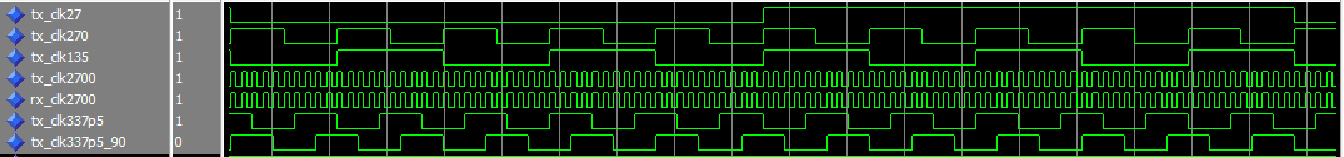
\includegraphics[width=1\textwidth]{./Figures/clks.png}
  %   \caption{Simulación del módulo nrz\_2\_nrzi.}\label{fig:clks}
  % \end{figure}

  El tiempo de bloqueo del receptor, especialmente en aplicaciones de
  comunicaciones o electrónica, se refiere al período requerido para que el
  receptor se estabilice y comience a funcionar correctamente después de ser
  activado o después de que se haya producido un cambio en la señal de entrada.

  \begin{figure}[h]
    \centering
    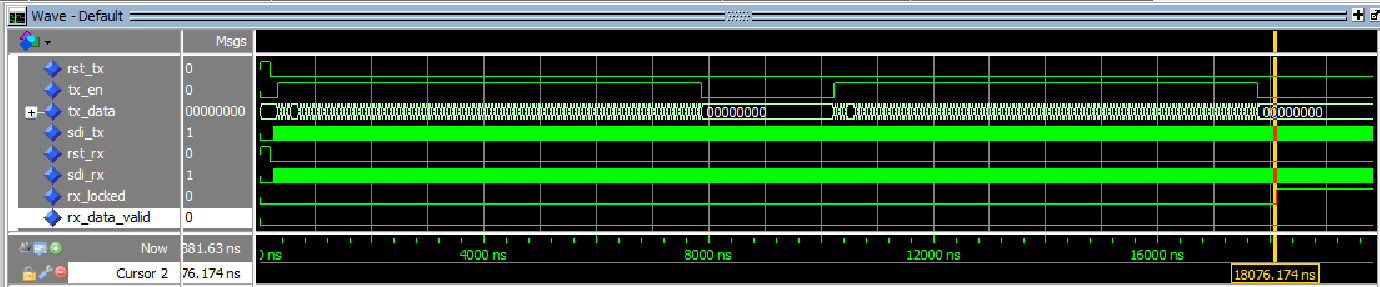
\includegraphics[width=1\textwidth]{./Figures/rx_lock_time.png}
    \caption{Simulación de tiempo hasta el bloqueo del receptor.}\label{fig:lock}
  \end{figure}

  El tiempo de bloqueo de 18 µs, que se ve en la figura~\ref{fig:lock} indica que el receptor puede adaptarse
  rápidamente a cambios, mientras que la latencia del trasmisor es inferior a 200 ns,
  por lo que es despreciable para el análisis y el tiempo que tarda en trasmitirse
  un mensaje entero es de un poco menos de 8 us, que da una referencia de que
  18 us es un tiempo muy reducido y satisfactorio para esta aplicación.
  Este tiempo de bloqueo puede ser un parámetro crítico
  cuando se evalúa la eficiencia de sistemas que necesitan sincronizarse con
  señales asincrónicas. Considerando que el tiempo que tarda un mensaje SD

  Con datos específicos o un contexto más detallado sobre la imagen o el
  sistema al que se aplica este tiempo de bloqueo, se puede ofrecer una interpretación
  más precisa o detallada sobre su importancia o impacto.

  El hecho de que los datos recibidos coincidan exactamente con los datos enviados,
  ver figura~\ref{fig:sd-full}, demuestra que la integridad de la señal se mantiene
  a lo largo del proceso de transmisión. Esto implica que el sistema es capaz de
  manejar las señales de video SD-SDI sin introducir errores, lo cual es crucial
  para aplicaciones profesionales de video donde la calidad y la precisión son críticas.

  \begin{figure}[h]
    \centering
    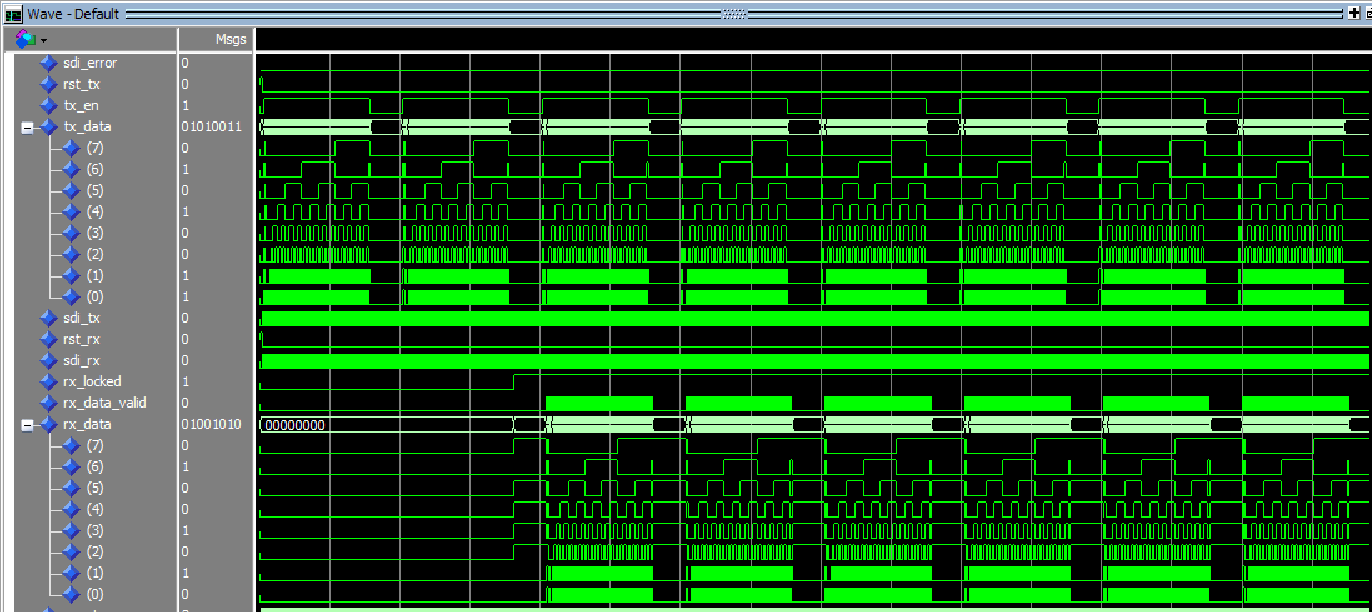
\includegraphics[width=1\textwidth]{./Figures/sdi_sd_full.png}
    \caption{Simulación del módulo en \textit{loopback}.}\label{fig:sd-full}
  \end{figure}

  La confirmación de que el transmisor y receptor pueden operar en \textit{loopback}
  con éxito es un fuerte indicador de la fiabilidad del sistema. Esto demuestra que
  tanto el módulo de transmisión y recepción están correctamente configurados y son
  capaces de manejar las especificaciones del estándar SD-SDI\@.

  Esta prueba valida el diseño del sistema de transmisión y recepción SD, asegurando
  que ambos componentes son compatibles y pueden trabajar juntos sin problemas.
  Previamente ambos se probaron con la misma configuración, pero conectándolos
  con el complementario del IP de Altera y funcionaron correctamente. Es una
  verificación crucial antes de proceder a fases más avanzadas de \textit{testing}
  o antes de desplegar el sistema en un entorno de producción. AL tratarse de una prueba
  que se configura de forma manual y como las mediciones se hacen de la misma forma, se optó
  por hacer solo la prueba con menos parámetros a configurar.

  En el proceso de desarrollo, un resultado exitoso en la prueba de \textit{loopback} facilita
  el diagnóstico y la resolución de problemas, ya que establece un punto de referencia
  de funcionamiento correcto. Cualquier desviación de este resultado en pruebas futuras
  puede ayudar a identificar problemas específicos con cambios en el diseño,
  configuración o en componentes individuales.

% TODO agregar y analiar las dos imagenes ya bajadas, la de lock itme y la de valid time

